\chapter{Machine learning algorithms comparison} \label{chap:methods}

%essayer d'autres noyaux pour SVM
%roc pour tous les scenariaux
%concatenate all datasets

%rappeler objectif
Before going further and analysing neural networks in order to create a hybrid machine learning algorithm for anomaly detection in the power distribution system presented in chapter \ref{chap:intro}, a deeper look at classical machine learning algorithms will be taken, in particular Random Forest, Support Vector Machine (SVM), NaïveBayes and multilayer perceptron. However this was done before in \cite{borges_hink_machine_2014-1} using the black-box model algorithms only. In their approach they used Weka \cite{witten_appendix_2017} in order to find the most performant algorithm among 7 they have chosen (OneR, NNge, Random Forest, Naïve Bayes, SVM, JRipper, Adaboost). 

This chapter shows an attempt to reproduce the results provided in \cite{borges_hink_machine_2014-1}, using two different machine learning toolkits (Weka and scikit-learn \cite{pedregosa_scikit-learn_2011}) in order to confirm the obtained results. That is why, first, these two toolkits will be presented, then the obtained results will be discussed.  

\section{Machine learning toolkits}
\subsection{Weka} \label{sec:weka_in_chap:methods}
%les parametres des algos, m par defaut
\textbf{Weka}, or more exactly \textbf{W}aikato \textbf{E}nvironment for \textbf{K}nowledge \textbf{A}nalysis, is an open source machine learning software developed at The University of Waikato in Hamilton, New Zealand and based on Java programming language. It is well known especially in academic environments and a lot of machine learning researches were conducted using it, one of them the mentioned before \cite{borges_hink_machine_2014-1}. It incorporates various machine learning tools: classifiers, regressors, visualizers, data pre-processor etc...

Weka is characterised by 3 main operating schemes. First, it can be run using a \textbf{graphical user interface} (GUI), enabling the user, even without deep knowledge in programming, to make machine learning experiments and analyse available classifiers. Second, more advanced users have the option to run all the available tools using a \textbf{command line}. Finally, Weka's tools can be \textbf{integrated directly into code in several programming languages (Java, Python, R, Spark)}, which enables even larger versatility.

\subsection{scikit-learn}
scikit-learn is an open-source machine learning \textbf{Python library} developed originally by David Cournapeau as a Google Summer of Code project and now it is maintained by a team of volunteers. It is well known in both academic and commercial environments, since it is used by many enterprises such as Spotify, Evernote, Booking.com, and research facilities like Inria or Télécom ParisTech \cite{noauthor_who_nodate}. It includes, just like Weka, various machine learning tools such as classifiers, regressors, data pre-processor etc... Its visualisation capabilities are limited, however there exist many additional Python packages for data visualisation such as YellowBrick, Eli5 and others... They will be further discussed in next chapter.

scikit-learn can be used only as an extension of Python language, what makes a bit harder for non experts to start working with it. However, since Python is an user friendly programming language and scikit-learn has a well made documentation, this toolkit is easy to use. Along with other Python packages, and especially pandas, scikit-learn is a very powerful, ergonomic and versatile solution for machine learning problems.  

It might be also interesting to mention that scikit-learn can be used within Weka after installing the appropriate add-on. This enables Weka users to use scikit-learn classifiers and regressors and run Python code just inside Weka's GUI.

\section{Used machine learning algorithms}
Before talking about the comparison of machine learning algorithms, the used classifiers are briefly described in this section in order to better understand how do they work. In parallel, values of classifiers' parameters used during all the tests are presented in tables \ref{tab:rf_param}, \ref{tab:svm_param} and \ref{tab:nb_param}, and, in majority, they represent the default values found in Weka, in order to reproduce the results from~\cite{borges_hink_machine_2014-1}.

\subsection{Random Forest} \label{sec:rf}
Random Forest, as the name indicates, is an \textbf{ensemble} of a given number of trees, and more exactly \textbf{decision trees}. This given number of trees is set using the parameter \textit{numIterations} in Weka and \textit{n\_estimators} in scikit-learn. Each of decision trees is created based on a randomly chosen set of features of the dataset. The number of features is given by the parameter \textit{numFeatures} in Weka and \textit{max\_features} in scikit-learn, which indicate the way it is calculated - in this case as the logarithm of base 2 of the number of features. 

On the other hand, decision trees represent a structure capable of determining the class of the predicted sample. It is composed of nodes connected to each other in a form of tree. Each node corresponds to a condition related to the features, for example if a particular feature is higher than a certain number. Each node, except the decision ones, has two child nodes corresponding to the answer as yes or no to the condition from from parent node. For each of two answers, particular classes are assigned, for example, given the case study in this work, yes answer can correspond to classes Attack and Natural and the answer no to class NoEvents. When running a tree on a particular sample, the nodes are followed given the answers on conditions, until arriving to the decision node. The class corresponding to this node is taken as the final output of the decision tree. The number of layers of nodes is called the depth of the tree and it is set using the parameter \textit{maxDepth} in both Weka and scikit-learn.

The choice of condition in a node is based on calculating \textbf{gini impurity} or \textbf{information gain} metric for each feature and determining, based on one of them, which feature has the biggest effect on the choice of the class. Gini impurity determines the probability of a feature being classified incorrectly when selected randomly, it is given by the equation:
\begin{equation}
    \text{Gini impurity} = 1 - \sum^n_{i=1} (p_i)^2,
\end{equation}
where n is the number of classes and $p_i$ the probability of the feature being classified for the class i. The information gain on the other hand, determines the quantity of information that the features gives about a particular class, it is calculated as:
\begin{equation}
    E(S) = \sum^n_{i=1} - p_i \log_2 p_i.
\end{equation}
Weka uses the information gain metric, while in scikit-learn it is possible to choose the metric using the parameter \textit{criterion}, which by default is set to gini impurity, which is less computationally complex.

The random forest, composed of a number of those decision trees, determines the class of a sample taking the class, which was chosen by the biggest amount of decision trees. In both Weka and scikit-learn, this classifier comes with more, less crucial parameters, which are all listed in table~\ref{tab:rf_param}.

\begin{table}[H]
    \footnotesize
    \centering
    \caption{Random Forest classifier parameters} \label{tab:rf_param}
    \begin{subtable}[t]{.5\linewidth}
        \caption{Weka \cite{noauthor_randomforest_nodate}}
        \centering
        \begin{tabular}{lr}\toprule
            Parameter & Value \\\midrule
            bagSizePercent & 100\\
            batchSize & 100 \\
            breakTiesRandomly & False \\
            calcOutOfBag & False \\
            computeAttributeImportance & False \\
            debug & False \\
            doNotCHeckCapabilities & False \\
            maxDepth & 0 \\
            numDecimalPlaces & 2 \\
            numExecutionSlots & 1 \\
            numFeatures & 0 \\
            numIterations & 100 \\
            outputOutOfBagComplexityStatistics & False \\
            printClassifiers & False \\
            seed & 1 \\
            storeOutOfBagPredictions & False \\\bottomrule
        \end{tabular}
    \end{subtable}%
    \begin{subtable}[t]{.5\linewidth}
        \caption{scikit-learn \cite{noauthor_sklearnensemblerandomforestclassifier_nodate}}
        \centering
        \begin{tabular}{lr}\toprule
            Parameter & Value \\\midrule
            n\_estimators & 100 \\
            criterion & "gini" \\
            max\_depth & None \\
            min\_samples\_split & 2 \\
            min\_samples\_leaf & 1 \\
            min\_weight\_fraction\_leaf & 0.0 \\
            max\_features & "log2" \\
            max\_leaf\_nodes & None \\
            min\_impurity\_decrease & 0.0 \\
            min\_impurity\_split & None \\
            bootstrap & True \\
            oob\_score & False \\
            n\_jobs & None \\
            random\_state & None \\
            verbose & 0 \\
            warm\_start & False \\
            class\_weight & None \\
            ccp\_alpha & 0.0 \\
            max\_samples & None \\\bottomrule
        \end{tabular}
    \end{subtable}%
\end{table}

\subsection{SVM}

SVM, or more exactly \textbf{Support Vector Machine}, is a classifier that creates an N-dimensional space, in which all the samples from the training dataset are put, and then divided, geometrically, into regions, where each region corresponds to one class. The N dimensions of this space corresponds to all the features of the datasets and their transformations (for example a square of one of the features). Those transformations are done using a kernel function which can be set in Weka and scikit-learn using the \textit{kernelType/kernel} parameter. Three kernel types are more commonly used: linear, polynomial and radial basis function (exponent based). The default kernel in both Weka and scikit-learn is radial basis function. Each type of kernel function comes with a set a parameters itself, like the degree in the case of polynomial and all of them can be set through the parameters of both used machine learning toolkits.

In fact, the transformations do not calculate additional dimensions for every sample, but calculate the distance between points in the N-dimensional space. This distance is mathematically defined as the \textbf{dot product} of the two points. The dot product on other hand is defined of the sum of products of coordinates for every dimension. 

The division is made by determining so called \textbf{hyperplane}, which for example in a 2D features spaces is just a line. The points from each class that are the closest to the hyperplane are called \textbf{support vector points}, from where comes the name of this classifier \cite{yadav_support_2018} \cite{noauthor_support_2014}. 

The algorithm is running within a set number of iterations (can be set within Weka and scikit-learn) dividing the training dataset to smaller tranches using the cross-validation technique. The goal is to find the hyperplane that way so the number of misclassified samples is the smallest in that particular iteration. 

SVM in Weka and scikit-learn comes additionally with other parameters than a:re listed on table~\ref{tab:svm_param}.

\begin{table}[H]
    \footnotesize
    \centering
    \caption{SVM classifier parameters} \label{tab:svm_param}
    \begin{subtable}[t]{.5\linewidth}
        \caption{Weka \cite{noauthor_libsvm_nodate}}
        \centering
        \begin{tabular}{lr}\toprule
            Parameter & Value \\\midrule
            SVMType & C-SVC (classification) \\
            batchSize & 100 \\
            cacheSize & 40.0 \\
            coef0 & 0.0 \\
            cost & 1.0 \\
            debug & False \\
            degree & 3 \\
            doNotCHeckCapabilities & False \\
            doNotReplaceMissingValues & False \\
            eps & 0.001 \\
            gamma & 0.0 \\
            kernelType & radial basis function\\
            loss & 0.1 \\
            modelFile & Weka-3-8-4 \\
            normalize & False \\
            nu & 0.5 \\
            numDecimalPlaces & 2 \\
            probabilityEstimates & True \\
            seed & 1 \\
            shrinking & True \\
            weights & \\\bottomrule
        \end{tabular}
    \end{subtable}%
    \begin{subtable}[t]{.5\linewidth}
        \caption{scikit-learn \cite{noauthor_sklearnsvmsvc_nodate}}
        \centering
        \begin{tabular}{lr}\toprule
            Parameter & Value \\\midrule
            C & 1.0 \\
            kernel & "rbf" \\
            degree & 3 \\
            gamma & "scale" \\
            coef0 & 0.0 \\
            shrinking & True \\
            probability & True \\
            tol & 1e-3 \\
            cache\_size & 7000 \\
            class\_weight & None \\
            verbose & False \\
            max\_iter & 1000 \\
            decision\_function\_shape & "ovr" \\
            break\_ties & False \\
            random\_state & None \\\bottomrule
        \end{tabular}
    \end{subtable}%
\end{table}
 
\subsection{NaïveBayes}
NaïveBayes is a classifier based on the \textbf{Bayes theorem}, which states that the probability of event A, given that the event B happened is equal to the product of the probability of B given that A occurred and the probability of A, divided by the probability of B:
\begin{equation}
    P(A|B) = \frac{P(B|A)\dot P(A)}{P(B)}.
\end{equation}
While the naivety of the algorithm is due to it does not taking into consideration the eventual relations between the features.

The NaïveBayes classifier can be both \textbf{multinomial} and \textbf{gaussian}. In the multinomial case the probabilities are calculated the classical way (number of occurrences over all samples), whereas in the gaussian case, the probabilities are taken from the gaussian distribution of a given event. For both Weka and scikit-learn the gaussian case were used.

The list of all the parameters available is listed on table \ref{tab:nb_param}, however they impact on how the algorithm works is marginal. 

\begin{table}[H]
    \footnotesize
    \centering
    \caption{NaïveBayes classifier parameters} \label{tab:nb_param}
    \begin{subtable}[t]{0.5\linewidth}
        \caption{weka \cite{noauthor_naivebayes_nodate}}
        \centering
        \begin{tabular}{lr}\toprule
            Parameter & Value \\\midrule
            batchSize & 100 \\
            debug & False \\
            displayModelInOldFormat & False \\
            doNotCHeckCapabilities & False \\
            numDecimalPlaces & 2 \\
            useKernelEstimator & False \\
            useSupervisedDiscretization & False\\\bottomrule
        \end{tabular}
    \end{subtable}%
    \begin{subtable}[t]{.5\linewidth}
        \caption{scikit-learn \cite{noauthor_sklearnnaive_bayesgaussiannb_nodate}}
        \centering
        \begin{tabular}{lr}\toprule
            Parameter & Value \\\midrule
            priors & None \\
            var\_smoothing & 1e-9 \\\bottomrule
        \end{tabular}
    \end{subtable}%
\end{table}

\subsection{Multilayer perceptron}
The multilayer perceptron is a classifier inspired by the structure of the human brain. It is constituted from a set of interconnected neurons, which are divided into at least 2 layers: input layer, $n$ hidden layers and output layer. Each layer consist of a number of neurons. The input layer has always a number of neurons equal to the number of features, and the output layer has always this number equal to the number of outputs of the problem. That is why, in the analysed case the input layer has 128 neurons and the output layer only one neuron corresponding to the status of the power plant (normal behaviour, natural fault, attack). Each of the mentioned neurons has a weight. The neurons are interconnected. The output of a neuron is considered as the input for the neurons of the following layer. Those neurons of the following layer calculates the weighted sum of the inputs and passes the results through a function, called activation function. The result obtained this way is considered as the output of the given neuron and goes to the following layer. The only exception is the input layer, which input is the values of features and its neurons just copy the input to the output \cite{patel_implementing_2020} \cite{noauthor_neural_nodate} \cite{stokfiszewski_soft_nodate}.

The training process consists in updating the weights of the neurons during a predefined number of iterations called epochs. Before starting the training process the initial weights $w_i$ values for hidden and output layers should be chosen. This choice can be done empirically or randomly. Moreover, a real positive number $\eta$ called training step must be fixed. In each epoch and for each training pattern, the weights are updated following the equation:
\begin{equation}
    w_i = w_i + \eta\cdot (z^{(\mu)}-y) \cdot x_i^{(\mu)},
\end{equation}
where $z^{(\mu)}$ is the desired output for the $\mu$-th training sample, $y$ is the neuron output (weighted sum passed through the activation function), $x_i^{(\mu)}$ is the neuron's input value for the same $\mu$-th training sample and $i$ indicates the neuron index in the trained layer. After each epoch, the training samples are shuffled \cite{stokfiszewski_soft_nodate}. 

The scikit-learn implementation of multilayer perceptron classifier is limited because it does not give a full control of each hidden layer and its activation function. It integrates however the possibility to determine the number of epochs called iterations and the training step called learning rate. All available parameters available are shown in table \ref{tab:mlp_param}. The implementation of MLP exists also in Weka, but it is as well limited, for this reason the analysis of its results will not be taken into consideration.

There exists multiple python frameworks offering much more flexibility when creating neural networks like PyTorch or Keras framework, which were created in order to offer the possibility to create complex neural networks able to be used in large-scale applications. Even the developers of scikit-learn state on their website \cite{noauthor_neural_nodate}:

\begin{quote}
    \textit{This implementation is not intended for large-scale applications. In particular, \mbox{scikit-learn} offers no GPU support.} 
\end{quote}

The mentioned frameworks will not be used in this work because this flexibility is not required in this case. However, it does not mean that it is not possible to make the results even better using those frameworks.

\begin{table}[H]
    \footnotesize
    \centering
    \caption[MLP classifier parameters in scikit-learn]{MLP classifier parameters in scikit-learn \cite{noauthor_sklearnneural_networkmlpclassifier_nodate}} \label{tab:mlp_param} 
    \begin{tabular}{lr}\toprule
        Parameter & Value \\\midrule
        hidden\_layer\_sizes & (20,) \\
        activation & 'relu' \\
        solver & 'adam' \\
        alpha & $0.0001$ \\
        batch\_size & 'auto' \\
        learning\_rate & 'constant' \\
        learning\_rate\_init & $0.001$ \\
        power\_t & $0.5$ \\
        max\_iter & 1000 \\
        shuffle & True \\
        random\_state & None \\
        tol & $1e-4$ \\
        verbose & False \\
        warm\_start & False \\
        momentum & $0.9$ \\
        nesterovs\_momentum & True \\
        early\_stopping & True \\
        validation\_fraction & $0.1$ \\
        beta\_1 & $0.9$ \\
        beta\_2 & $0.999$ \\
        epsilon & $1e-8$ \\
        n\_iter\_no\_change & $10$ \\
        max\_fun & $15000$ \\\bottomrule
    \end{tabular}
\end{table}

\section{Metrics for classifiers comparison}
All those classifiers give predictions that can be divided into 4 main groups. Assuming for a moment, for illustration purposes, that normal fault class is positive and attack class is negative, it could be differentiated between:
\begin{itemize}
    \item true positive predictions (\textbf{tp}): correct prediction of the normal fault class,
    \item true negative predictions (\textbf{tn}): correct prediction of the attack class,
    \item false positive predictions (\textbf{fp}): incorrect prediction of normal fault class,
    \item false negative predictions (\textbf{fn}): incorrect prediction of attack class.
\end{itemize}
For that two classes, several metrics can be defined, that will be useful to compare between the used classifiers: 
\begin{itemize}
    \item \textbf{accuracy}: ratio of correct classifications over the total number of samples, or in other words:
    \begin{equation}
        \text{accuracy} = \frac{tp + tn}{tp + tn + fp + fn}
    \end{equation}
    \item \textbf{precision}:  ratio of correct classifications for a particular class over all classifications that indicated that class, or:
    \begin{equation}
        \text{precision} = \frac{tp}{tp + fp}
    \end{equation}
    \item \textbf{recall}: ratio of correct classifications for a particular class, over all samples corresponding for this class, or:
    \begin{equation}
        \text{recall} = \frac{tp}{tp + fn}
    \end{equation}
    \item \textbf{f-measure}: weighted average of precision and recall given by the equation: 
    \begin{equation*}
        \text{f-measure} = 2 \times \frac{\mathrm{precision} \times \mathrm{recall}}{\mathrm{precision} + \mathrm{recall}}.
    \end{equation*}
\end{itemize}

Given that those metrics work only with binary problems with a positive and a negative class, for multiclass problems the \textbf{accuracy is always calculated as the ratio of true classifications over all classifications}, however for precision, recall and f-measure, the average is calculated, and that in 3 different ways \cite{shmueli_multi-class_2020}:

\begin{itemize}
    \item \textbf{micro} average: the metrics are determined globally by calculating true positives as all correct predictions, false negatives and false positives as all incorrect predictions (assuming two classes A and B, when A is misclassified as B is a false positive for A, and in the same time a false negative for B). In this case precision, recall, f-measure and accuracy have exactly the same value,
    \item \textbf{macro} average: the metrics are calculated for each class, the concerned class is considered as positive, while the sum of others as negative. Then their arithmetic mean value is calculated,
    \item \textbf{weighted} average: the metrics are calculated for each class, then it calculates their weighted average value by the number of true instances for each class.
\end{itemize}

scikit-learn supports the calculation of precision, recall and f-measure in the 3 different ways explicitly, however in Weka only for f-measure all 3 are available, while for precision and recall there is the choice between the generic ones and the weighted averages. The generic ones the most probably correspond to the macro average, since, after some tests, the obtained values for those metrics are not the same. The exact information about the nature of those averages could not be found in Weka's documentation.

\section{Comparison results}
In order to reproduce the results presented in \cite{borges_hink_machine_2014-1}, Weka version 3.8.4 and scikit-learn version 0.23.1, running on Anaconda 3.18.11 with Python 3.7.6.final.0, were used. SVM in Weka comes from a package untitled \textit{libsvm} available for this toolkit. The results are displayed in the same order as in \cite{borges_hink_machine_2014-1}, thus, the accuracy was presented on figures \ref{fig:weka_acc3}, \ref{fig:weka_acc2} and \ref{fig:weka_accall} for the three class, binary and all 37 class cases respectively. Then, the precision, recall and f-measure can be found on figures \ref{fig:prec}, \ref{fig:recall} and \ref{fig:f1}. For f-measure the scikit-learn plot is not displayed because Weka differentiates between micro, macro and weighted averages and a generic value for f-measure. The generic value does not correspond by value to the other averages.  

\begin{figure}[H]
    \centering
    \begin{subfigure}[t]{0.4\textwidth}
        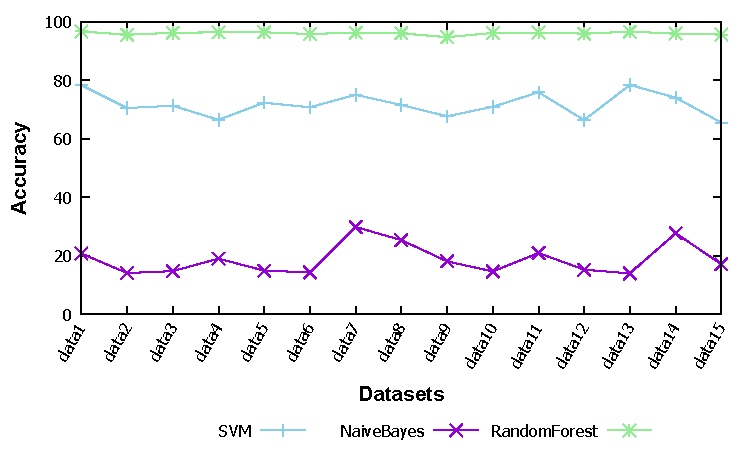
\includegraphics[width=\linewidth]{images/weka_accuracy3}
        \caption{Our attempt - Weka}
    \end{subfigure}%
    \begin{subfigure}[t]{0.4\textwidth}
        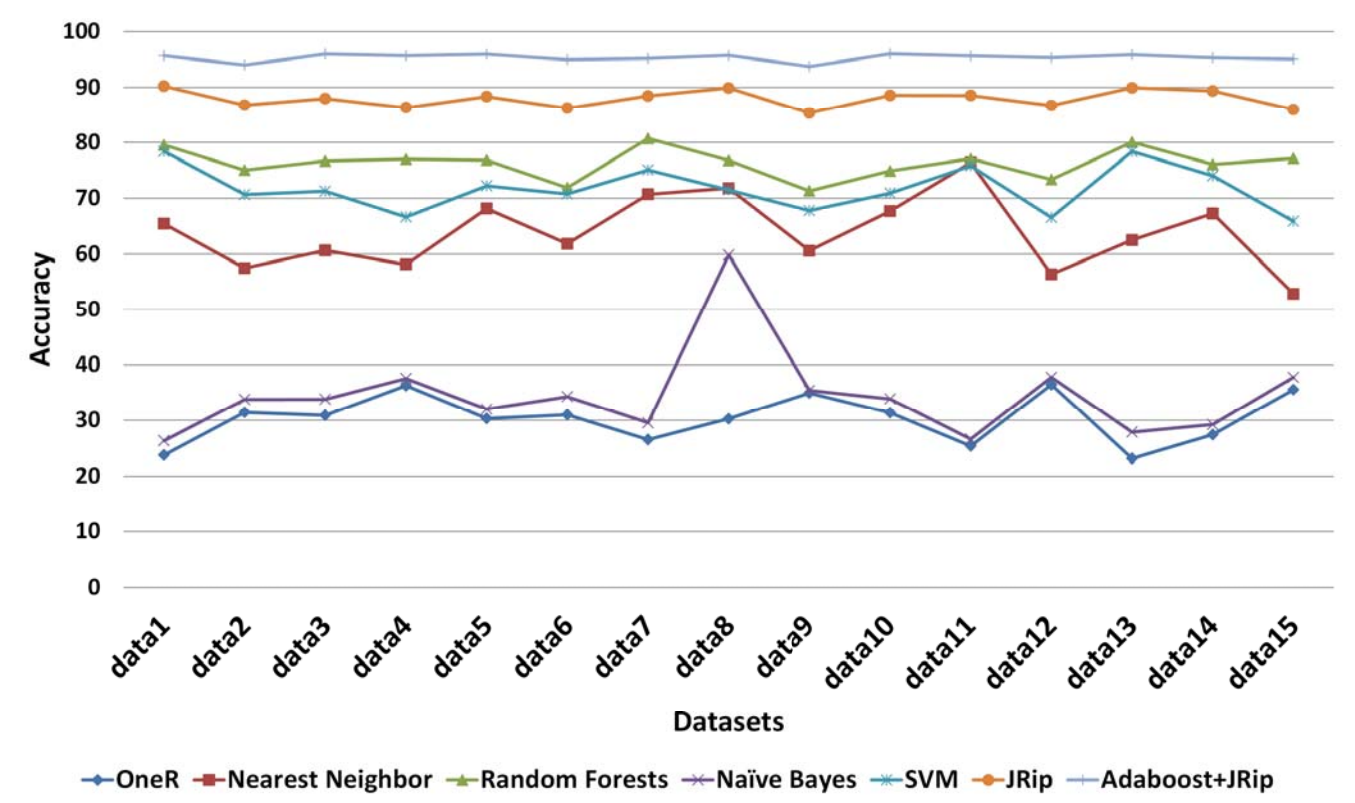
\includegraphics[width=\linewidth]{images/weka_accuracy3_cite.png}
        \caption{Original results \cite{borges_hink_machine_2014-1}}
    \end{subfigure}
    \begin{subfigure}[t]{0.4\textwidth}
        \includegraphics[width=\linewidth, page = 2]{images/accuracy}
        \caption{Our attempt - scikit-learn}
    \end{subfigure}
    \caption{Accuracy for three-class datasets}
    \label{fig:weka_acc3}
\end{figure}

\begin{figure}[H]
    \centering
    \begin{subfigure}[t]{0.4\textwidth}
        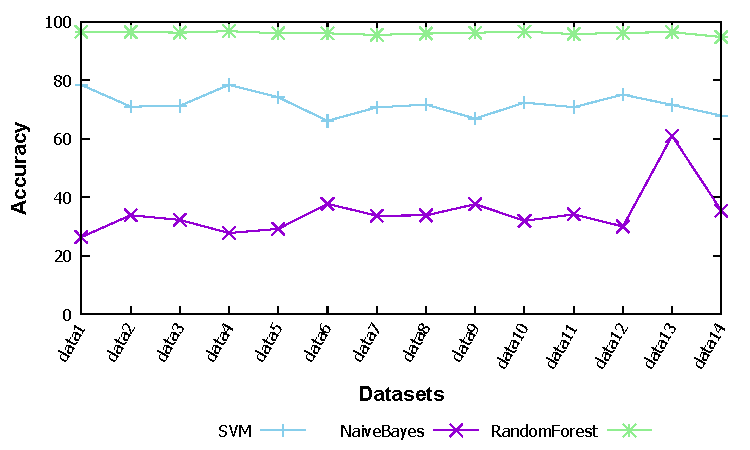
\includegraphics[width=\linewidth]{images/weka_accuracy2}
        \caption{Our attempt - Weka}
    \end{subfigure}%
    \begin{subfigure}[t]{0.4\textwidth}
        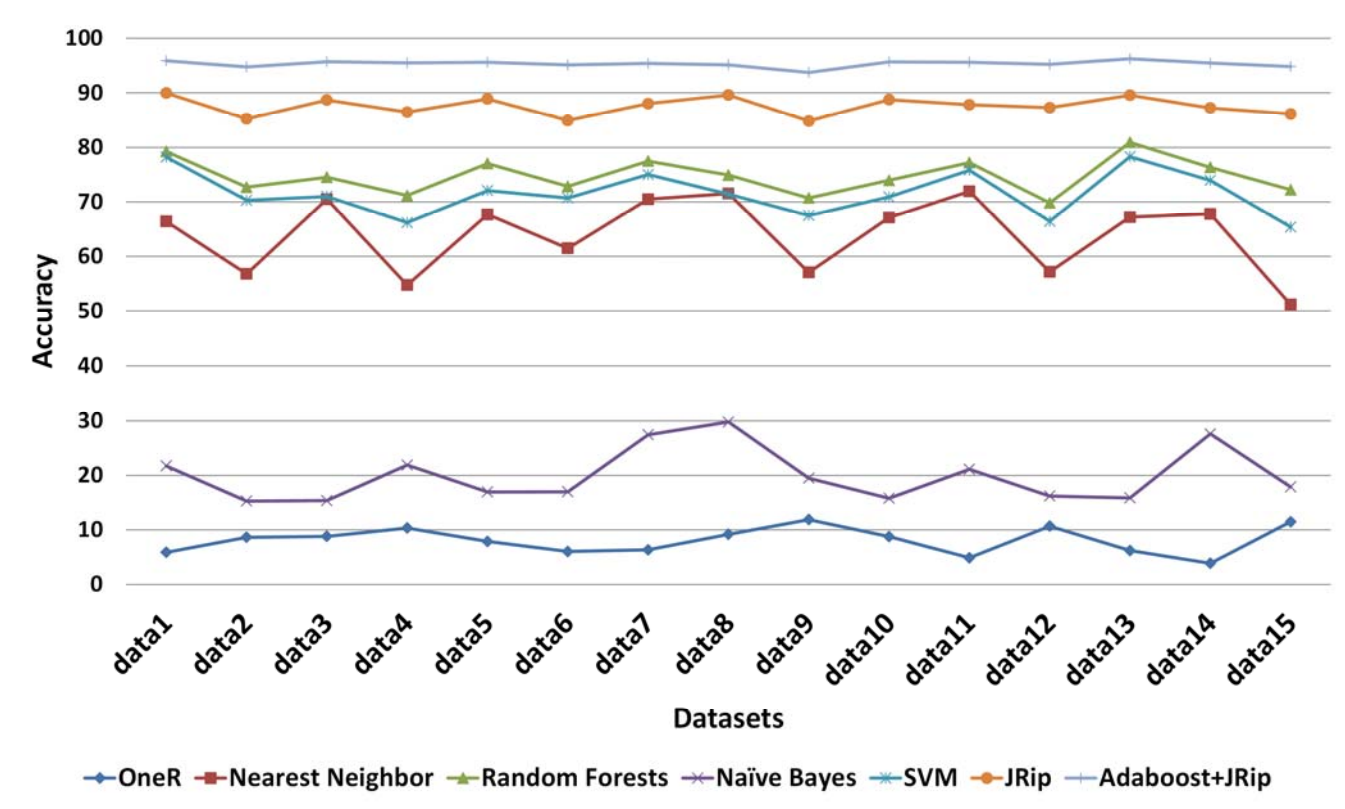
\includegraphics[width=\linewidth]{images/weka_accuracy2_cite.png}
        \caption{Original results \cite{borges_hink_machine_2014-1}}
    \end{subfigure}    
    \begin{subfigure}[t]{0.4\textwidth}
        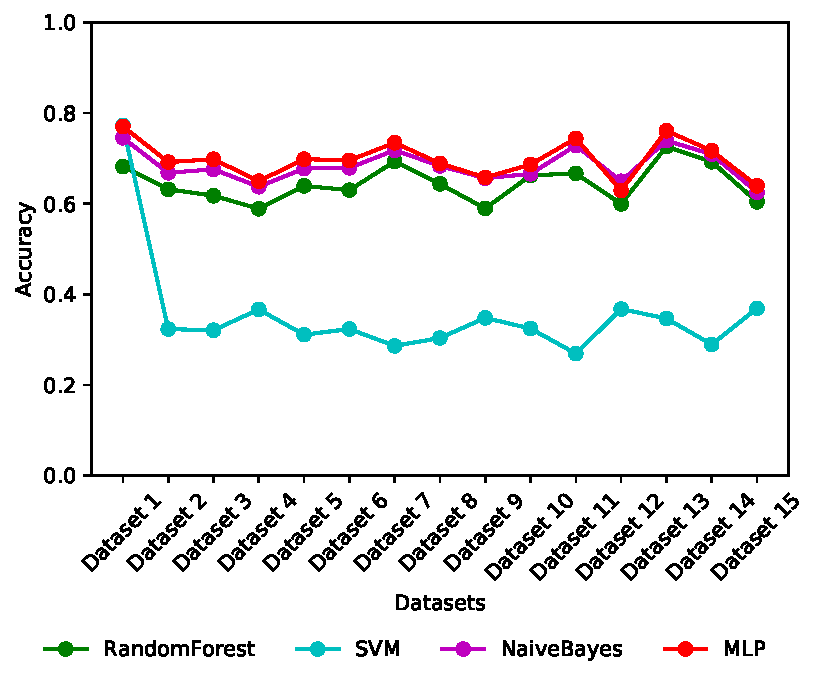
\includegraphics[width=\linewidth, page = 1]{images/accuracy}
        \caption{Our attempt - scikit-learn}
    \end{subfigure}
    \caption{Accuracy for binary datasets}
    \label{fig:weka_acc2}
\end{figure}

\begin{figure}[H]
    \centering
    \begin{subfigure}[t]{0.4\textwidth}
        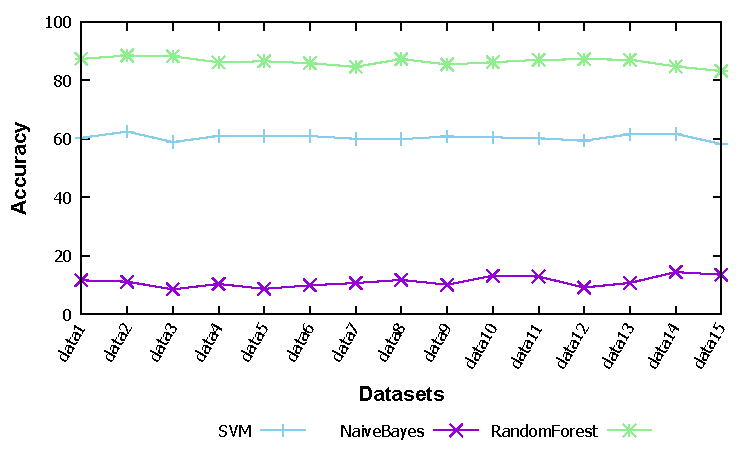
\includegraphics[width=\linewidth]{images/weka_accuracyall}
        \caption{Our attempt - Weka}
    \end{subfigure}%
    \begin{subfigure}[t]{0.4\textwidth}
        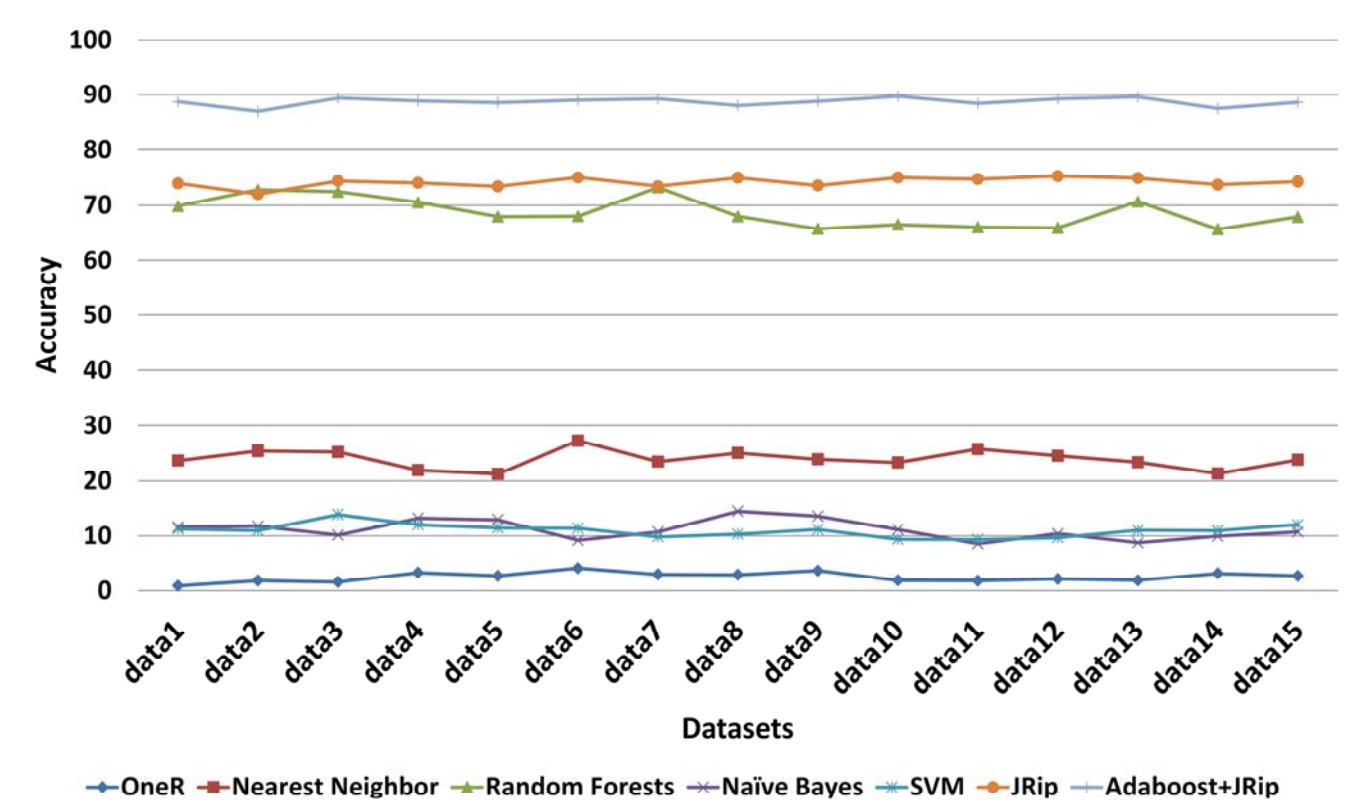
\includegraphics[width=\linewidth]{images/weka_accuracyall_cite.png}
        \caption{Original results \cite{borges_hink_machine_2014-1}}
    \end{subfigure}
    \begin{subfigure}[t]{0.4\textwidth}
        \includegraphics[width=\linewidth, page = 3]{images/accuracy}
        \caption{Our attempt - scikit-learn}
    \end{subfigure}
    \caption{Accuracy for multiclass datasets}
    \label{fig:weka_accall}
\end{figure}

\begin{figure}[H]
    \centering
    \begin{subfigure}[t]{0.4\textwidth}
        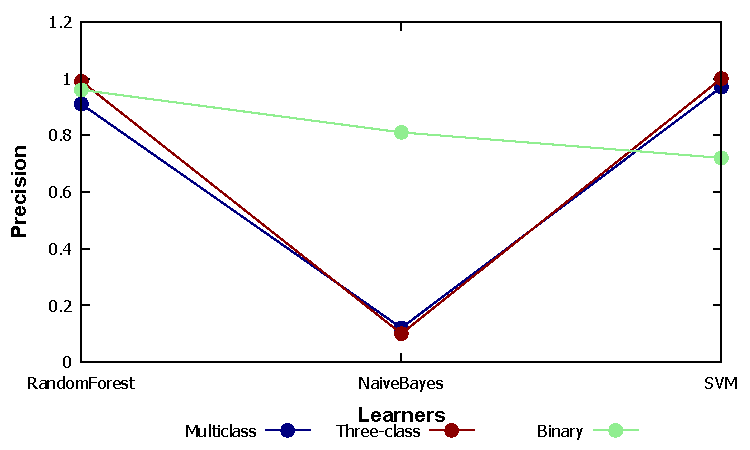
\includegraphics[width=\linewidth]{images/weka_precision}
        \caption{Our attempt - Weka}
    \end{subfigure}%
    \begin{subfigure}[t]{0.4\textwidth}
        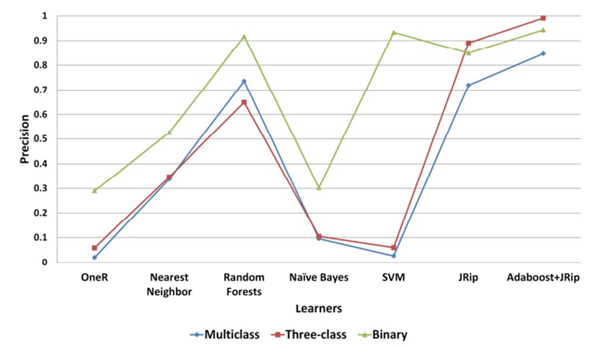
\includegraphics[width=\linewidth]{images/weka_precision_cite.png}
        \caption{Original results \cite{borges_hink_machine_2014-1}}
    \end{subfigure}
    \begin{subfigure}[t]{0.4\textwidth}
        \includegraphics[width=\linewidth, page = 2]{images/precision}
        \caption{Our attempt - scikit-learn}
    \end{subfigure}
    \caption{Precision}
    \label{fig:prec}
\end{figure}

\begin{figure}[H]
    \centering
    \begin{subfigure}[t]{0.4\textwidth}
        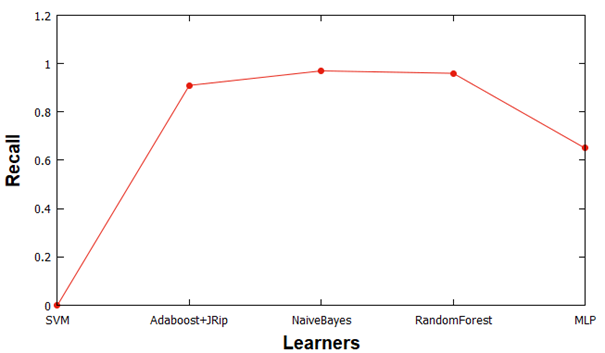
\includegraphics[width=\linewidth]{images/weka_recall}
        \caption{Our attempt - Weka}
    \end{subfigure}%
    \begin{subfigure}[t]{0.4\textwidth}
        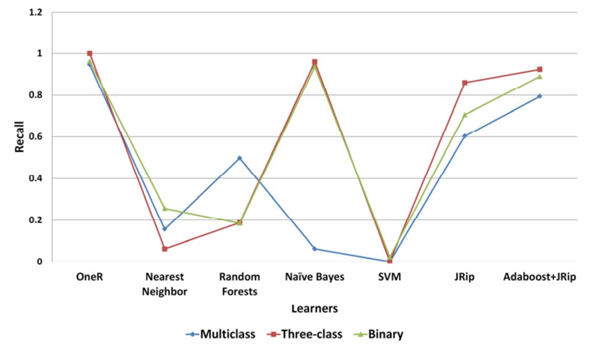
\includegraphics[width=\linewidth]{images/weka_recall_cite.png}
        \caption{Original results \cite{borges_hink_machine_2014-1}}
    \end{subfigure}
    \begin{subfigure}[t]{0.4\textwidth}
        \includegraphics[width=\linewidth, page = 2]{images/recall}
        \caption{Our attempt - scikit-learn}
    \end{subfigure}
    \caption{Recall}
    \label{fig:recall}
\end{figure}

\begin{figure}[H]
    \centering
    \begin{subfigure}[t]{0.5\textwidth}
        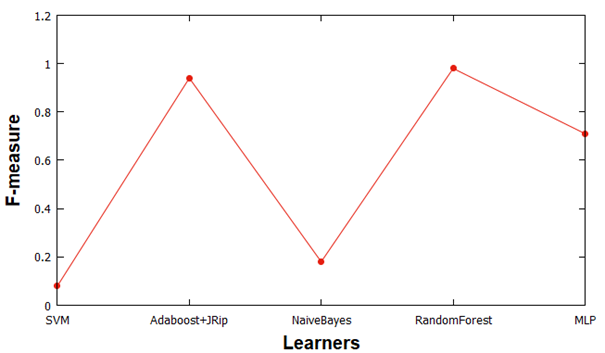
\includegraphics[width=\linewidth]{images/weka_f1}
        \caption{Our attempt - Weka}
    \end{subfigure}%
    \begin{subfigure}[t]{0.5\textwidth}
        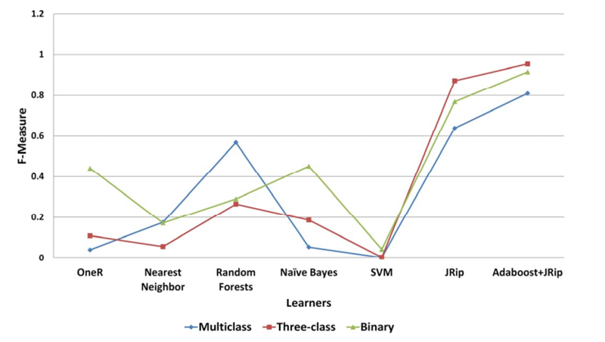
\includegraphics[width=\linewidth]{images/weka_f1_cite.png}
        \caption{Original results \cite{borges_hink_machine_2014-1}}
    \end{subfigure}
    \caption{F-measure}
    \label{fig:f1}
\end{figure}

The accuracies in the three-class case are quite similar on the three plots, except SVM in scikit-learn, which show a huge discrepancy of accuracy between datasets. Moreover, a remarkably higher values of accuracy for Random Forest classifier are observed in the attempt using Weka, compared to other plots.

In the binary and multiclass cases, the Random Forest classifier in the attempts using Weka always shows higher values compared to other plots. Scikit-learn, on other hand, for Random Forest classifier, gives results similar to those made by \cite{borges_hink_machine_2014-1}. For SVM classifier, the variance this time, in the plots made by scikit-learn, is remarkably less important and the values oscillate around a constant value. For the binary case, this value is about 0.3, while in Weka the obtained value is 0.75 (comparable to the original results in \cite{borges_hink_machine_2014-1}). On the other hand, in the multiclass case, it oscillates around 0.1, like it is the case in the results from \cite{borges_hink_machine_2014-1}. In the attempt made in Wake the accuracy is much higher at about 0.6. For the NaïveBayes classifier the results are comparable, except the results obtained in scikit-learn in the binary case.

Concerning the other metrics, Random Forest classifier shows values close to 1 in both Weka and scikit-learn, while the original results for recall and f-measure show small values. For the rest of classifiers the results are generally totally different between attempts, with some exceptions (like SVM recall with Weka in three-class case compared to \cite{borges_hink_machine_2014-1}, or also SVM recall, but with scikit-learn and in multiclass case compared to \cite{borges_hink_machine_2014-1}).

It can be concluded from here, that the results from \cite{borges_hink_machine_2014-1} were successfully reproduced in Weka in the three-class and binary cases, however for multiclass the reproduction of the results failed. Scikit-learn, on other hand, gives different results than Weka despite using the same algorithms with the same set of parameters. The more efficient classifier is certainly Random Classifier, especially when using Weka. However, MLP classifier gives also quite good results.

Moreover to get more information about the behaviour of the classifiers the f-measure macro, micro and weighted averages were calculated, along with precision and recall weighted averages. The results are shown on figures \ref{fig:f1_macro}, \ref{fig:f1_micro}, \ref{fig:f1_weight}, \ref{fig:prec_weight} and \ref{fig:recall_weight} respectively. The values of f-measure micro, weighted and precision weighted for NaïveBayes classifier for multiclass case could not be calculated for unknown reason. These metrics were not presented in \cite{borges_hink_machine_2014-1}.

\begin{figure}[H]
    \centering
    \begin{subfigure}[t]{0.5\textwidth}
        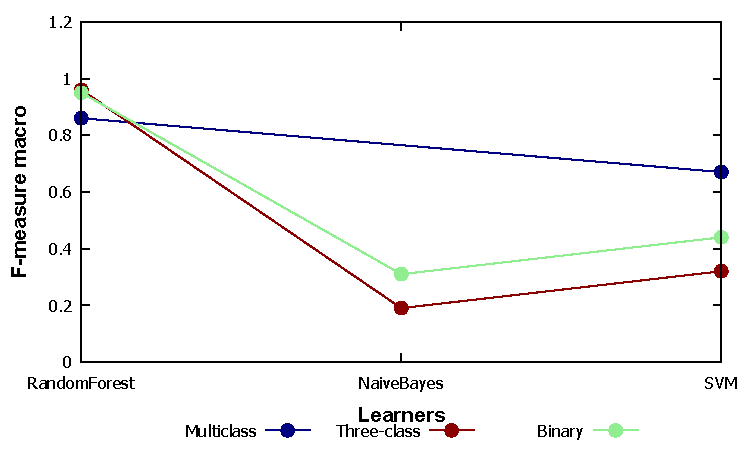
\includegraphics[width=\linewidth]{images/weka_f1macro}
        \caption{Weka}
    \end{subfigure}%
    \begin{subfigure}[t]{0.42\textwidth}
        \includegraphics[width=\linewidth, page = 2]{images/fmeasure}
        \caption{scikit-learn}
    \end{subfigure}
    \caption{F-measure macro}
    \label{fig:f1_macro}
\end{figure}

\begin{figure}[H]
    \centering
    \begin{subfigure}[t]{0.5\textwidth}
        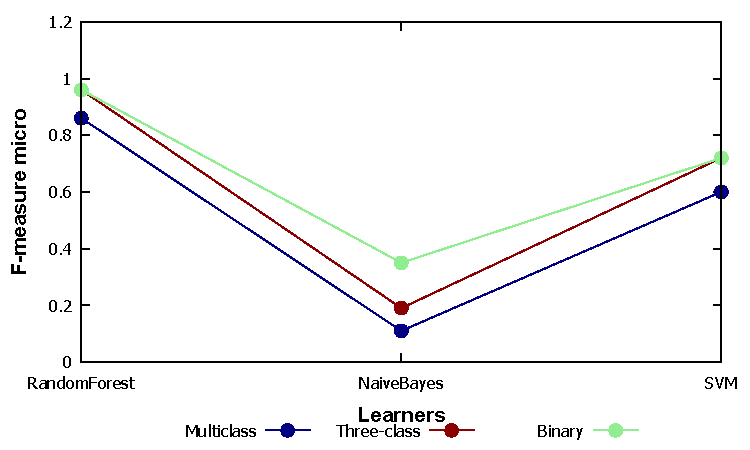
\includegraphics[width=\linewidth]{images/weka_f1micro}
        \caption{Weka}
    \end{subfigure}%
    \begin{subfigure}[t]{0.42\textwidth}
        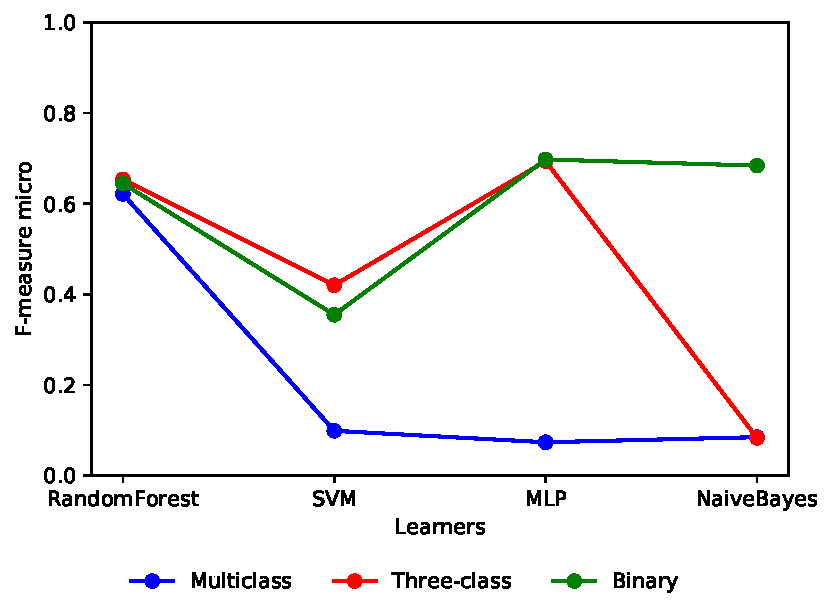
\includegraphics[width=\linewidth, page = 1]{images/fmeasure}
        \caption{scikit-learn}
    \end{subfigure}
    \caption{F-measure micro}
    \label{fig:f1_micro}
\end{figure}

\begin{figure}[H]
    \centering
    \begin{subfigure}[t]{0.5\textwidth}
        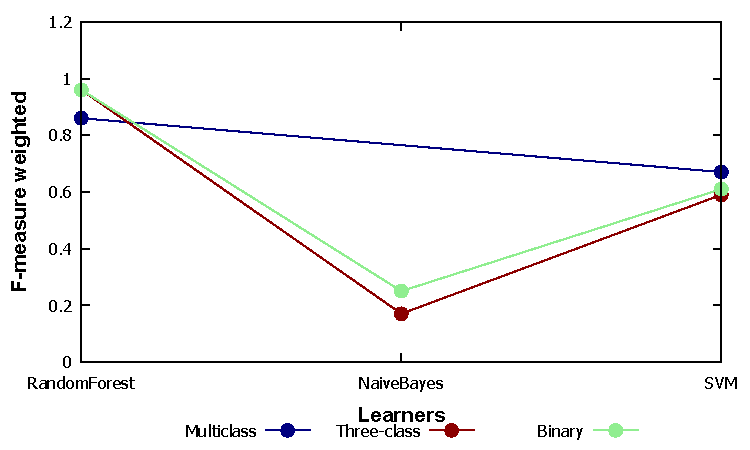
\includegraphics[width=\linewidth]{images/weka_f1weight}
        \caption{Weka}
    \end{subfigure}%
    \begin{subfigure}[t]{0.42\textwidth}
        \includegraphics[width=\linewidth, page = 3]{images/fmeasure}
        \caption{scikit-learn}
    \end{subfigure}
    \caption{F-measure weighted}
    \label{fig:f1_weight}
\end{figure}


\begin{figure}[H]
    \centering
    \begin{subfigure}[t]{0.5\textwidth}
        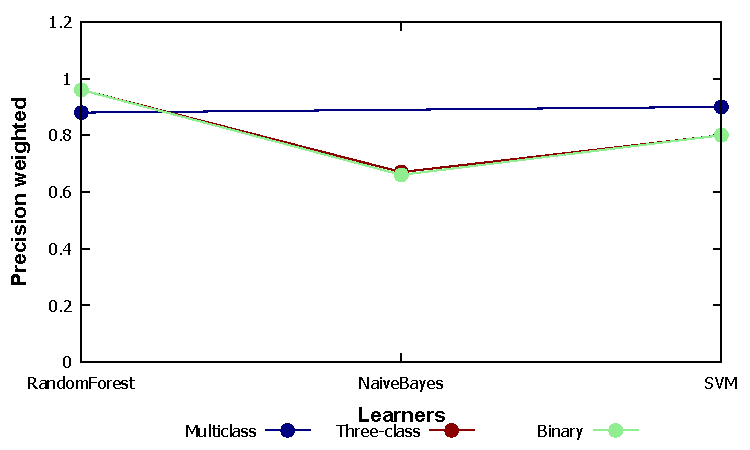
\includegraphics[width=\linewidth]{images/weka_precweight}
        \caption{Weka}
    \end{subfigure}%
    \begin{subfigure}[t]{0.42\textwidth}
        \includegraphics[width=\linewidth, page = 3]{images/precision}
        \caption{scikit-learn}
    \end{subfigure}
    \caption{Precision weighted}
    \label{fig:prec_weight}
\end{figure}

\begin{figure}[H]
    \centering
    \begin{subfigure}[t]{0.5\textwidth}
        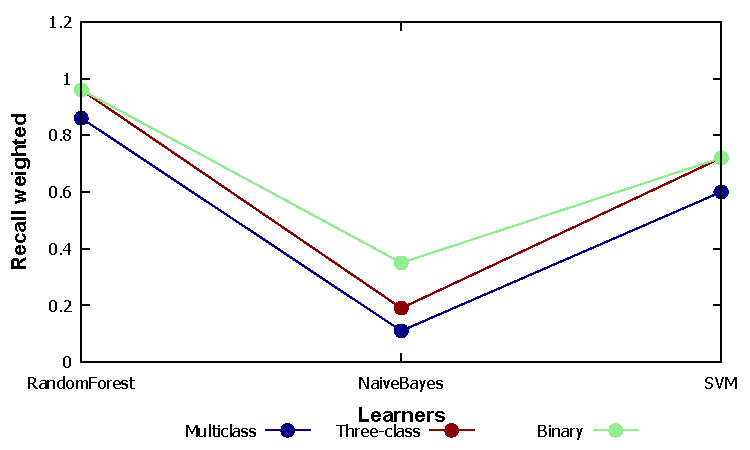
\includegraphics[width=\linewidth]{images/weka_recallweight}
        \caption{Weka}
    \end{subfigure}%
    \begin{subfigure}[t]{0.42\textwidth}
        \includegraphics[width=\linewidth, page = 3]{images/recall}
        \caption{scikit-learn}
    \end{subfigure}
    \caption{Recall weighted}
    \label{fig:recall_weight}
\end{figure}

It would be hard to say that the obtained results in Weka and scikit-learn are similar, except the three-class case, where the results are quite similar. These results confirm once more time that Weka and scikit-learn tend to produce different results and that the best classifier is Random Forest, followed by MLP, especially in binary and three-class cases.

Since the results for three-class and binary cases were comparable and the three-class case gives more information about the status of the system, in what follows, the focus will be on the three-class case.

\section{scikit-learn further methods' analysis}

In addition to all that, scikit-learn enables the user to plot the receiver operating characteristic (ROC) curves for each class and the confusion matrix. The ROC curve represents the plot od true positive rate when the false positive rate changes. It is based on the prediction probabilities for each class given for each tested sample. Those predictions can be provided in two different ways:
\begin{itemize}
    \item concatenation of these probabilities for each cross-validation iteration,
    \item determination of probabilities for preselected test dataset values.
\end{itemize} 
The confusion matrix on the other hand shows the normalized number (over the total number of samples) of predicted values of each class for each class. The results are illustrated on figures \ref{fig:ROCCM_RF}, \ref{fig:ROCCM_SVM}, \ref{fig:ROCCM_NB} and \ref{fig:ROCCM_MLP}.

\begin{figure}[H]
    \centering
    \begin{subfigure}[t]{0.33\textwidth}
        \centering
        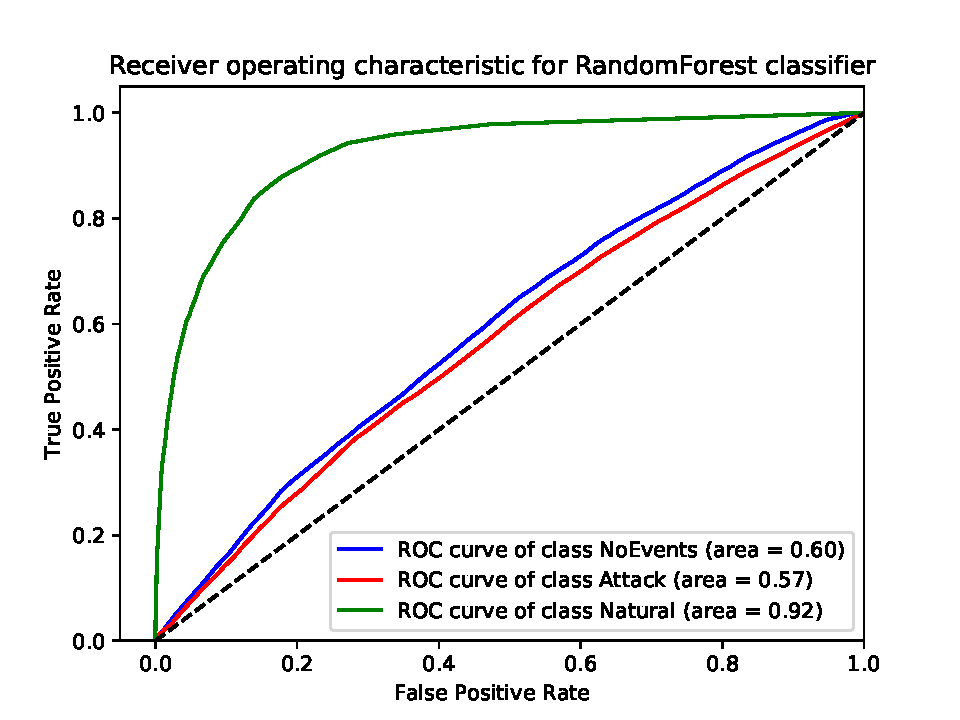
\includegraphics[page=1, width=\linewidth]{images/results_scikit/RandomForest}
        \caption{ROC Curve - cross-validation}
        \label{fig:scikit_RF_ROC}
    \end{subfigure}
    \begin{subfigure}[t]{0.33\textwidth}
        \centering
        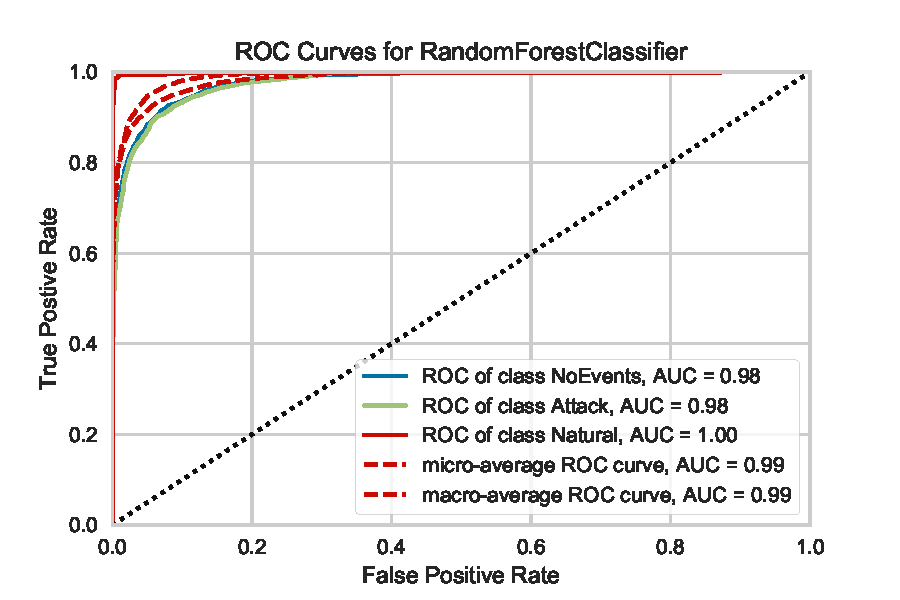
\includegraphics[page=1, width=\linewidth]{images/roc_3c}
        \caption{ROC Curve}
        \label{fig:scikit_RF_ROC}
    \end{subfigure}
    \begin{subfigure}[t]{0.3\textwidth}
        \centering
        \includegraphics[page=2, width=\linewidth, trim= 0 50 0 100, clip]{images/results_scikit/RandomForest}
        \caption{Confusion Matrix}
        \label{fig:scikit_RF_CM}
    \end{subfigure}
    \caption{Random Forest ROC curve and confusion matrix}
    \label{fig:ROCCM_RF}
\end{figure}

\begin{figure}[H]
    \centering
    \begin{subfigure}[t]{0.33\textwidth}
        \centering
        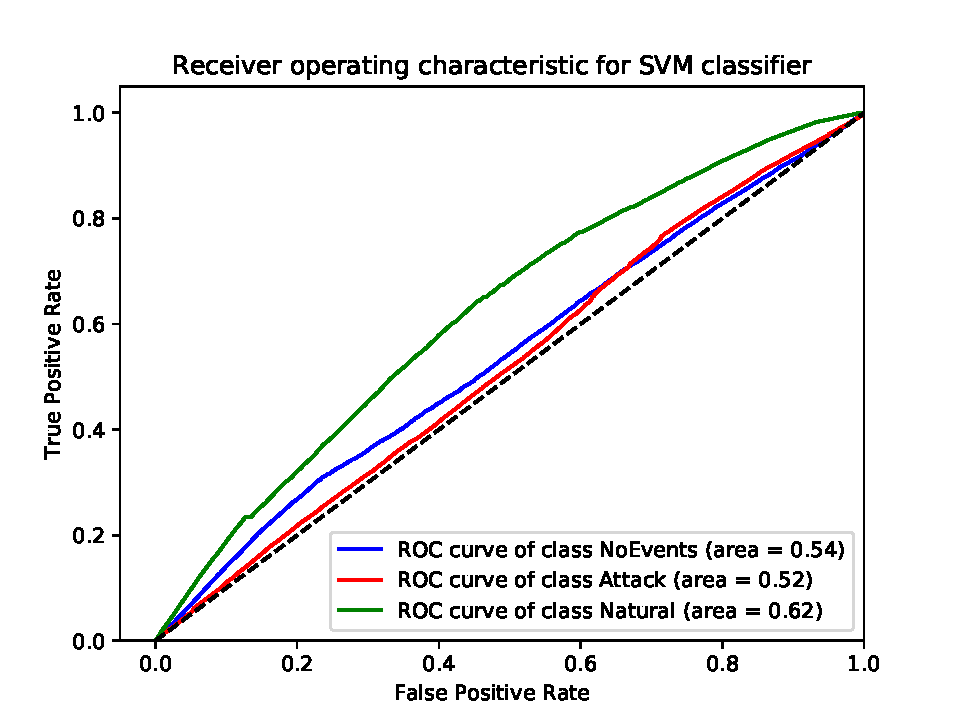
\includegraphics[page=1, width=\linewidth]{images/results_scikit/SVM}
        \caption{ROC Curve - cross-validation}
        \label{fig:scikit_SVM_ROC}
    \end{subfigure}
    \begin{subfigure}[t]{0.33\textwidth}
        \centering
        \includegraphics[page=2, width=\linewidth]{images/roc_3c}
        \caption{ROC Curve}
        \label{fig:scikit_RF_ROC}
    \end{subfigure}
    \begin{subfigure}[t]{0.3\textwidth}
        \centering
        \includegraphics[page=2, width=\linewidth, trim= 0 50 0 100, clip]{images/results_scikit/SVM}
        \caption{Confusion Matrix}
        \label{fig:scikit_SVM_CM}
    \end{subfigure}
    \caption{SVM ROC curve and confusion matrix}
    \label{fig:ROCCM_SVM}
\end{figure}

\begin{figure}[H]
    \begin{subfigure}[t]{0.33\textwidth}
        \centering
        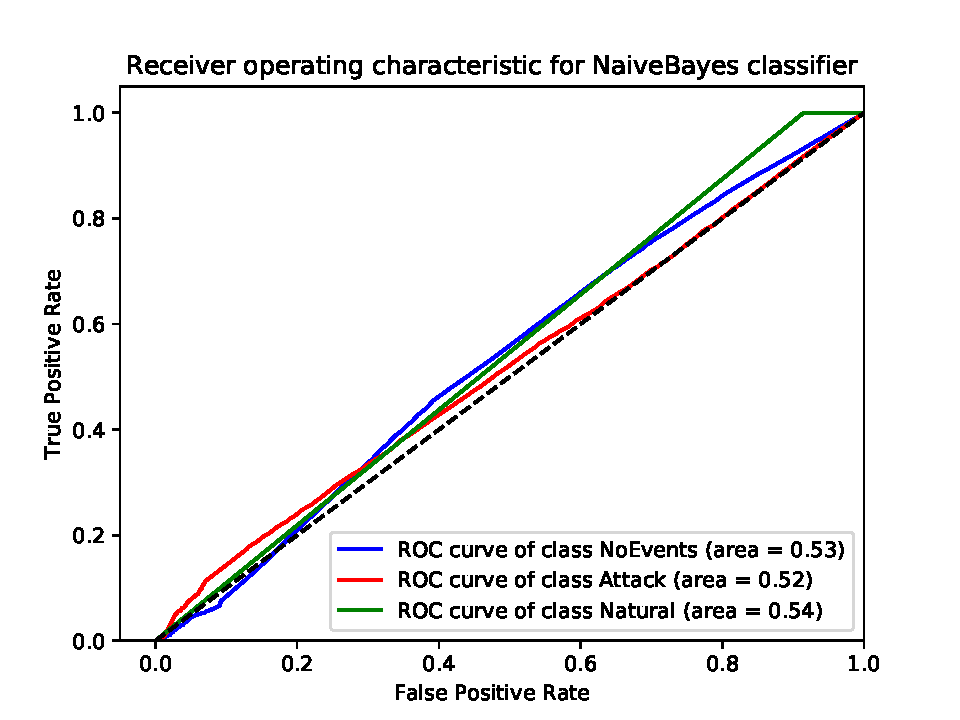
\includegraphics[page=1, width=\linewidth]{images/results_scikit/NaiveBayes}
        \caption{ROC Curve - cross-validation}
        \label{fig:scikit_NB_ROC}
    \end{subfigure}
    \begin{subfigure}[t]{0.33\textwidth}
        \centering
        \includegraphics[page=4, width=\linewidth]{images/roc_3c}
        \caption{ROC Curve}
        \label{fig:scikit_RF_ROC}
    \end{subfigure}
    \begin{subfigure}[t]{0.3\textwidth}
        \centering
        \includegraphics[page=2, width=\linewidth, trim= 0 50 0 100, clip]{images/results_scikit/NaiveBayes}
        \caption{Confusion Matrix}
        \label{fig:scikit_NB_CM}
    \end{subfigure}
    \caption{Naïve Bayes ROC curve and confusion matrix}
    \label{fig:ROCCM_NB}
\end{figure}

\begin{figure}[H]
    \begin{subfigure}[t]{0.33\textwidth}
        \centering
        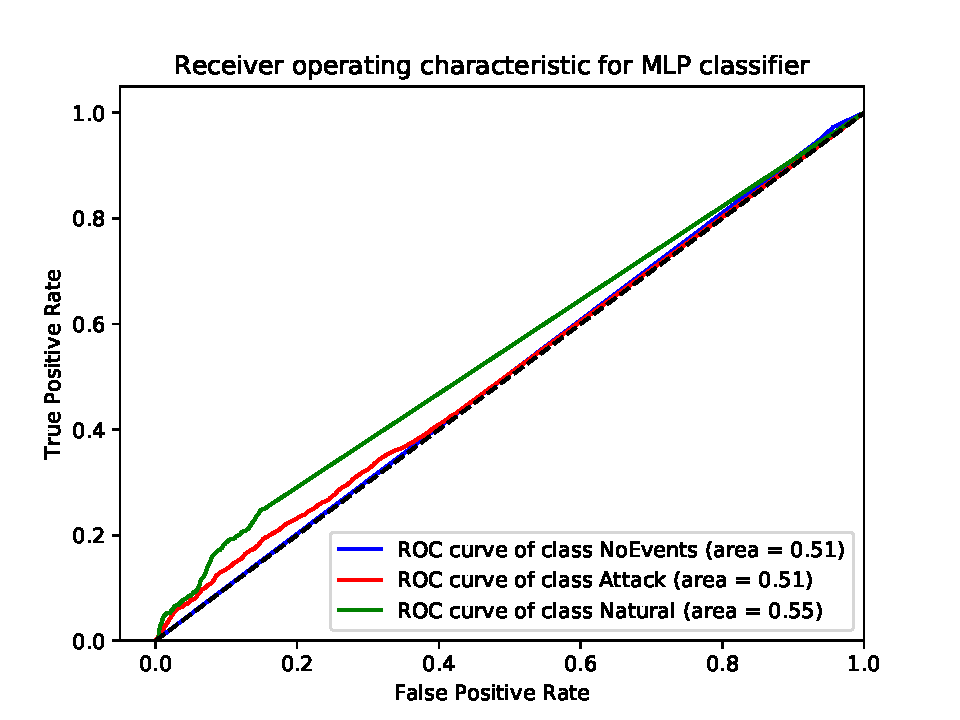
\includegraphics[page=1, width=\linewidth]{images/results_scikit/MLP}
        \caption{ROC Curve - cross-validation}
        \label{fig:scikit_MLP_ROC}
    \end{subfigure}
    \begin{subfigure}[t]{0.33\textwidth}
        \centering
        \includegraphics[page=3, width=\linewidth]{images/roc_3c}
        \caption{ROC Curve}
        \label{fig:scikit_RF_ROC}
    \end{subfigure}
    \begin{subfigure}[t]{0.3\textwidth}
        \centering
        \includegraphics[page=2, width=\linewidth, trim= 0 50 0 100, clip]{images/results_scikit/MLP}
        \caption{Confusion Matrix}
        \label{fig:scikit_MLP_CM}
    \end{subfigure}
    \caption{MLP ROC curve and confusion matrix}
    \label{fig:ROCCM_MLP}
\end{figure}

The previous figures show that Random Forest classifier has the higher capacities to distinguish between the occurrence of each class, or it's absence. It's visible on both ROC curves and the confusion matrix, where the highest number of predictions is shown for the true positives for each class. SVM tends to predict only NoEvents and Attacks but does not really succeed in distinguishing between them. Naïve Bayes fails to make true predictions, it considers everything of class natural. Finally MLP, it succeeds in determining the class NoEvents, but does not distinguish over classes almost at all, despite the high accuracy (it is due because of the huge number of samples of class NoEvents).

The two methods of plotting the ROC curve does not give exactly the same results, however the conclusions remain the same in both cases. This fact may be due to a slightly different set of test data used for its creation.

Given this analysis, it can be deducted that Random Forest algorithm acts the best, and that is why it will be adapted in next chapters, in which, at first, an analysis of features and their importance will be made. However a deeper look at the amelioration of MLP, in order to succeed in differentiation between the classes, will be also made later.

